There are several types of Malware that can be used to compromise a network or
a computer.The propagation of a malware can also happen through social
engineering, being phishing one of the most common examples \citep{greenbergSandwormNewEra2019}.
This lab objective is to discover and research different types of specific
malwares.

\section{Zeus Gameover}
\label{s:Zeus-Gameover}
One of the most famous malware is Zeus Gameover. Zeus is a trojan that spreads
itself through emails with malicious attachments \citep{wikipediaGameoverZeuS2021}.
This malware will then generate zombies that sit in an IRC server managed by a
server administrator. This process is a continue and infinite loop and makes the
battle against the botnets really hard \citep{firatInevitableBattleBotnets2020}.
Zeus uses anAdobe Reader BMP/RLE heap corruption vulnerability CVE-2013-2729 that
causes a buffer overflow to cause a DoS that crashes the daemon and execute
malicious code \citep{ismailEffectsFeatureSelection2021}.
In the case of Zeus, most of the time, a PDF file is used to initialise
everything and start the new botnet. It will use the vulnerabilities of the
reader to declare previously where the shellcode is not even hidden, and that
can be easily decrypted \citep{eternalSpammedCVE20132729PDF2013}. These
discoveries are made using a python tool named peepdf that analyse a pdf file.
The principal scope of the botnet is to steal banking informations where the
victims are deprived of their money when the amount is worth to be taken \citep{
knowbe4GameoverZeusGOZ2020}. GOZ uses high TCP and UDP ports to spread itself.

\begin{figure}[H]
  \centering
  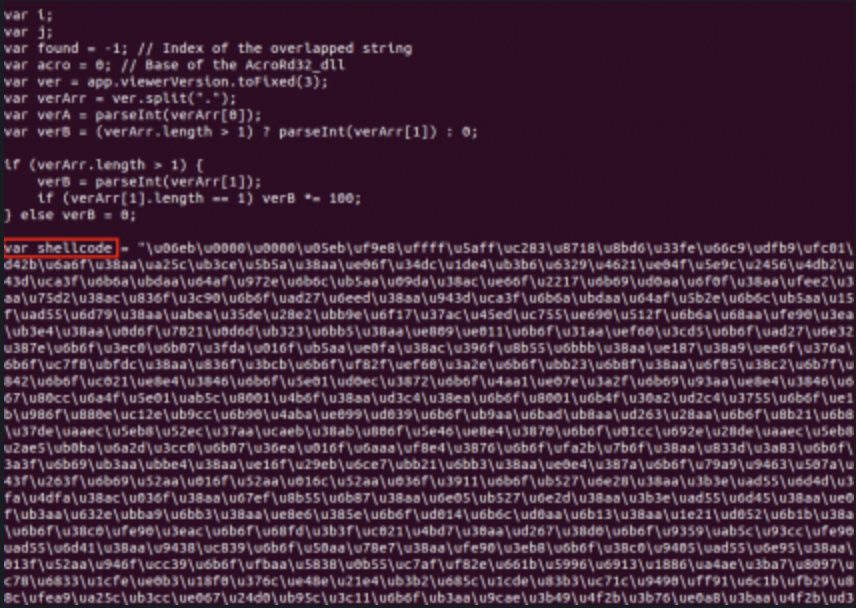
\includegraphics[width=0.5\textwidth]{figures/shellcode-zeus}
  \caption{Shellcode Zeus Gameover}
  \label{f:shellcode-zeus}
\end{figure}

\section{WannaCry}
\label{s:WannaCry}
WannaCry is a self-propagating ransomware that encrypts the victims' data on
outdated Microsoft platforms. It is known that the malware will also the user to pay a
ransom in Bitcoin or lose the data forever \citep{qianICMLA201716th2017}. This ransomware
propagates through a specific SMB protocol vulnerability that and needs NetBIOS
and SMB ports open \citep{nhsWannaCryRansomwareUsing2017}. One of the most
significant casualties of the attack has been the NHS, vulnerable to out-of-date
operative systems such as Windows XP that Microsoft no longer supported with
updates \citep{qianICMLA201716th2017}. Every system affected by this malware will look for
devices that takes inbound traffic on low TCP ports such as 135, 139 and 445
that are used by the SMB protocol.

\section{SQL Slammer}
\label{s:SQL-Slammer}
SQL Slammer has been released in the early hours of January 26 A worm takes
advantage of bugs to create copies of itself from local to network nodes. In
this case, SQL Slammer uses a buffer overflow vulnerability in the Microsoft SQL
Server and is remotely exploitable through the UDP 1434 port and its
vulnerability identifier is CVE-2002-0649 \citep{cveCVE200206492009}. SQL
Slammer has been one of the most fast spread worm in the history of internet as
it was scanning more than 55 million systems per second in the first three
minutes when it has been released and infected 90\% of exploitable hosts within
ten minutes. The spread was 250 times faster than Code Red
\citep{hoarTrendsCybercrimeDark2005}.

\begin{figure}[ht]
  \centering
  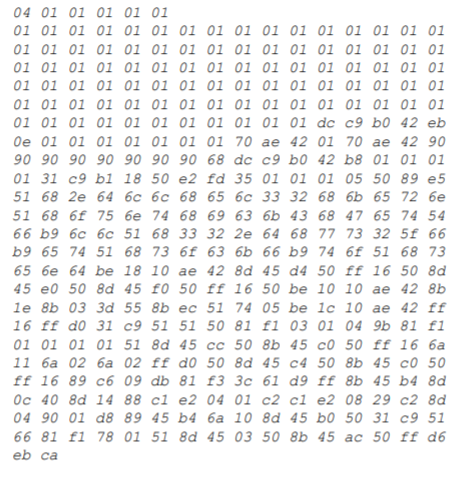
\includegraphics[width=0.5\textwidth]{figures/sql-slammer}
  \caption{SQL Slammer 376 bytes ASCII}
  \label{f:sql-slammer}
\end{figure}

\section{Conclusion}
\label{s:Week2-Conclusion}
There are many malware that, even though they have been released in the early
days of the spread of the internet, are still present, meaning that it is very
hard to find a way to fight them. Patches are very important to fix some
vulnerabilities, but at the same time, they can introduce new ones. Botnets are
still very predominant in today world, and IRC is still being used to manage
them in a very efficient way. Criminals are always finding new ways to exploit
machines to improve their security, such as encryptions and obfuscations while
hiding in the dark web. This lab has imprinted in me the awareness that
everything is exploitable and nothing is safe if it's exposed on the internet.
